% Foliensatz: "AFu-Kurs nach DJ4UF" von DK0TU, Amateurfunkgruppe der TU Berlin
% Lizenz: CC BY-NC-SA 3.0 de (http://creativecommons.org/licenses/by-nc-sa/3.0/de/)
% Autoren: Sebastian Lange <dl7bst@dk0tu.de>
% Korrekturen: Lars Weiler <dc4lw@darc.de>

\documentclass[aspectratio=169]{beamer}

\usepackage[ngerman]{babel} % deutsche Worttrennung etc.
\usepackage[utf8]{inputenc} % UTF8 Text

\usepackage[super, comma, numbers, square, sort]{natbib}

\usepackage{hyperref}       % Hyperref Package für bessere Referenzen (todo)
\hypersetup{
	colorlinks=false,       %   false: boxed links; true: colored links
    %linkcolor=white,       %   color of internal links (change box color with linkbordercolor)
    citecolor=red,          %   color of links to bibliography
    filecolor=white,        %   color of file links
    urlcolor=blue           %   color of external links
}

\usepackage{multirow}
\usepackage{wasysym}  % Math Symbols like \permil
%\usepackage{colortbl}
%\usepackage{subscript}
%\usepackage{caption}
%\usepackage{setspace}
%\usepackage{xcolor}        % benutze CodeListe

% Footnote
%\usepackage{hanging}
%
%\setbeamertemplate{footnote}{%
%  \hangpara{2em}{1}%
%  \makebox[2em][l]{\insertfootnotemark}\footnotesize\insertfootnotetext\par%
%}


%\usepackage{pgf}
%\usepackage{tikz}
%\usetikzlibrary{arrows,automata}
%\usetikzlibrary{positioning}
%
%\tikzset{
%    state/.style={
%           rectangle,
%           rounded corners,
%           draw=black, very thick,
%           minimum height=2em,
%           minimum width=2pt,
%           inner sep=2pt,
%           text centered,
%           },
%}

%\usepackage{listings}
%\lstset{basicstyle=\small, numberstyle=\tiny, extendedchars=true, numbers=left, numbersep=5pt}
%\lstset{showtabs=false, showspaces=false, showstringspaces=false}
%%\lstset{backgroundcolor=\color{white!75!lightgray}, , frame=single}
%%\lstset{backgroundcolor=\color{white}}
%%\lstset{backgroundcolor=none}
%\lstset{keywordstyle=\color{blue!50!gray},  identifierstyle=\color{black}}
%\lstset{commentstyle=\color{green!50!gray}, stringstyle=\color{red!50!gray}}
%\lstset{language=C, fontadjust=true, tabsize=2, breaklines=true}
%\lstset{backgroundcolor=\color{white!75!lightgray}, caption=\lstname, frame=single}
%\lstset{emphstyle=\color{black}\fbox}
%
%% Keine "Listing:"-Caption
%\captionsetup{labelformat=empty,labelsep=none}
%
%% für mathematische Umgebungen
%\usepackage{amsmath,amsfonts,amssymb}
%
%\lstdefinestyle{Bash}{
%language=Bash,
%frame=single,
%rulecolor=\color{black},
%backgroundcolor=\color{gray!50},
%keywordstyle=\color{black},
%identifierstyle=,
%commentstyle=\color{black},
%stringstyle=\color{magenta!65!white},
%showstringspaces=false,
%basicstyle=\footnotesize\ttfamily\color{black},
%numbers=none,
%breaklines=true,
%captionpos=b
%}

%\usepackage{listings}
%
%\lstdefinestyle{basic}{
%    captionpos=t,%
%    basicstyle=\footnotesize\ttfamily,%
%    numberstyle=\tiny,%
%    numbers=left,%
%    stepnumber=1,%
%    frame=single,%
%    showspaces=false,%
%    showstringspaces=false,%
%    showtabs=false,%
%    %
%    keywordstyle=\color{blue},%
%    identifierstyle=,%
%    commentstyle=\color{gray},%
%    stringstyle=\color{magenta}%
%}



% fließende Boxen haben keinen Abstand
%\fboxsep0mm

% inkludiere Creative Commons Helper
%%%%%%%%%%%%%%%%%%%%%%%%%%%%%%%%%%%%%%%%%%%%%%%%%%%%%%%%%%%%%%%%
%% ccBeamer 0.1, 2007-07-02                                   %%
%% Written by Sebastian Pipping <webmaster@hartwork.org>      %%
%% ---------------------------------------------------------- %%
%% Licensed under Creative Commons Attribution-ShareAlike 3.0 %%
%% http://creativecommons.org/licenses/by-sa/3.0/             %%
%%%%%%%%%%%%%%%%%%%%%%%%%%%%%%%%%%%%%%%%%%%%%%%%%%%%%%%%%%%%%%%%


%% Images
\newcommand{\CcImageBy}[1]{%
	
\includegraphics[scale=#1]{texdata/creative_commons/cc_by_30.pdf}%
}
\newcommand{\CcImageCc}[1]{%
	
\includegraphics[scale=#1]{texdata/creative_commons/cc_cc_30.pdf}%
}
\newcommand{\CcImageDevNations}[1]{%
	
\includegraphics[scale=#1]{texdata/creative_commons/cc_dev_nations_30.pdf}%
}
\newcommand{\CcImageNc}[1]{%
	
\includegraphics[scale=#1]{texdata/creative_commons/cc_nc_30.pdf}%
}
\newcommand{\CcImageNd}[1]{%
	
\includegraphics[scale=#1]{texdata/creative_commons/cc_nd_30.pdf}%
}
\newcommand{\CcImagePd}[1]{%
	
\includegraphics[scale=#1]{texdata/creative_commons/cc_pd_30.pdf}%
}
\newcommand{\CcImageSa}[1]{%
	
\includegraphics[scale=#1]{texdata/creative_commons/cc_sa_30.pdf}%
}
\newcommand{\CcImageSampling}[1]{%
	
\includegraphics[scale=#1]{texdata/creative_commons/cc_sampling_30.pdf}%
}
\newcommand{\CcImageSamplingPlus}[1]{%
	
\includegraphics[scale=#1]{texdata/creative_commons/cc_sampling_plus_30.pdf}%
}


%% Groups
\newcommand{\CcGroupBy}[2]{% zoom, gap
	\CcImageCc{#1}\hspace*{#2}\CcImageBy{#1}%
}
\newcommand{\CcGroupByNc}[2]{% zoom, gap
	\CcImageCc{#1}\hspace*{#2}\CcImageBy{#1}\hspace*{#2}\CcImageNc{#1}%
}
\newcommand{\CcGroupByNcNd}[2]{% zoom, gap
	\CcImageCc{#1}\hspace*{#2}\CcImageBy{#1}\hspace*{#2}\CcImageNc{#1}\hspace*{#2}\CcImageNd{#1}%
}
\newcommand{\CcGroupByNcSa}[2]{% zoom, gap
	\CcImageCc{#1}\hspace*{#2}\CcImageBy{#1}\hspace*{#2}\CcImageNc{#1}\hspace*{#2}\CcImageSa{#1}%
}
\newcommand{\CcGroupByNd}[2]{% zoom, gap
	\CcImageCc{#1}\hspace*{#2}\CcImageBy{#1}\hspace*{#2}\CcImageNd{#1}%
}
\newcommand{\CcGroupBySa}[2]{% zoom, gap
	\CcImageCc{#1}\hspace*{#2}\CcImageBy{#1}\hspace*{#2}\CcImageSa{#1}%
}
\newcommand{\CcGroupDevNations}[2]{% zoom, gap
	\CcImageCc{#1}\hspace*{#2}\CcImageDevNations{#1}%
}
\newcommand{\CcGroupNcSampling}[2]{% zoom, gap
	\CcImageCc{#1}\hspace*{#2}\CcImageNc{#1}\hspace*{#2}\CcImageSampling{#1}%
}
\newcommand{\CcGroupPd}[1]{% zoom
	\CcImagePd{#1}%
}
\newcommand{\CcGroupSampling}[1]{% zoom
	\CcImageSampling{#1}%
}
\newcommand{\CcGroupSamplingPlus}[1]{% zoom
	\CcImageSamplingPlus{#1}%
}


%% Text
\newcommand{\CcLongnameBy}{Attribution}
\newcommand{\CcLongnameByNc}{Attribution-NonCommercial}
\newcommand{\CcLongnameByNcNd}{Attribution-NoDerivs}
\newcommand{\CcLongnameByNcSa}{Attribution-NonCommercial-ShareAlike}
\newcommand{\CcLongnameByNd}{Attribution-NoDerivs}
\newcommand{\CcLongnameBySa}{Attribution-ShareAlike}

\newcommand{\CcNote}[1]{% longname
	This work is licensed under the \textit{Creative Commons #1 3.0 License}.%
}


% generelles Thema auswählen
\usetheme{Goettingen} %Berlin spart ohne Sidebar allerdings angenehm Platz
% AnnArbor | Antibes | Bergen | Berkeley | Berlin | Boadilla | boxes | CambridgeUS | Copenhagen | Darmstadt | default | Dresden | Frankfurt | Goettingen | Hannover | Ilmenau | JuanLesPins | Luebeck | Madrid | Malmoe | Marburg | Montpellier | PaloAlto | Pittsburgh | Rochester | Singapore | Szeged | Warsaw

% Farben wählen
\usecolortheme{beetle}
% beaver | beetle | crane | default | dolphin | dove | fly | lily | orchid | rose | seagull | seahorse | sidebartab | structure | whale | wolverine

% Setze alle Farben auf Grau und Weiß
%\definecolor{craneorange}{RGB}{64,64,64}
%\definecolor{craneblue}{RGB}{255,255,255}

% Schriftart wählen
\usefonttheme{default}
% default | professionalfonts | serif | structurebold | structureitalicserif | structuresmallcapsserif

% Innere Themen(Kopf-, Fuß-, Sidebar usw)
%\useinnertheme{default}
\useinnertheme{circles}
% default | inmargin | rectangles | rounded | circles

% Äußere Themen (Anordnung der inneren, grenzen der Folien etc.)
\useoutertheme{infolines}
% default | infolines | miniframes | shadow | sidebar | smoothbars | smoothtree | split | tree

% Deaktiviere Navigations-Symbole ({} -> leer)
\setbeamertemplate{navigation symbols}{}
%\setbeamertemplate{navigation symbols}{\large \ifnum \insertframenumber <10 0\fi\insertframenumber/\inserttotalframenumber\vspace*{0.2ex}}

% Zeige ein Hintergrundbild
\setbeamertemplate{background canvas}{
        \hspace*{-2.0cm}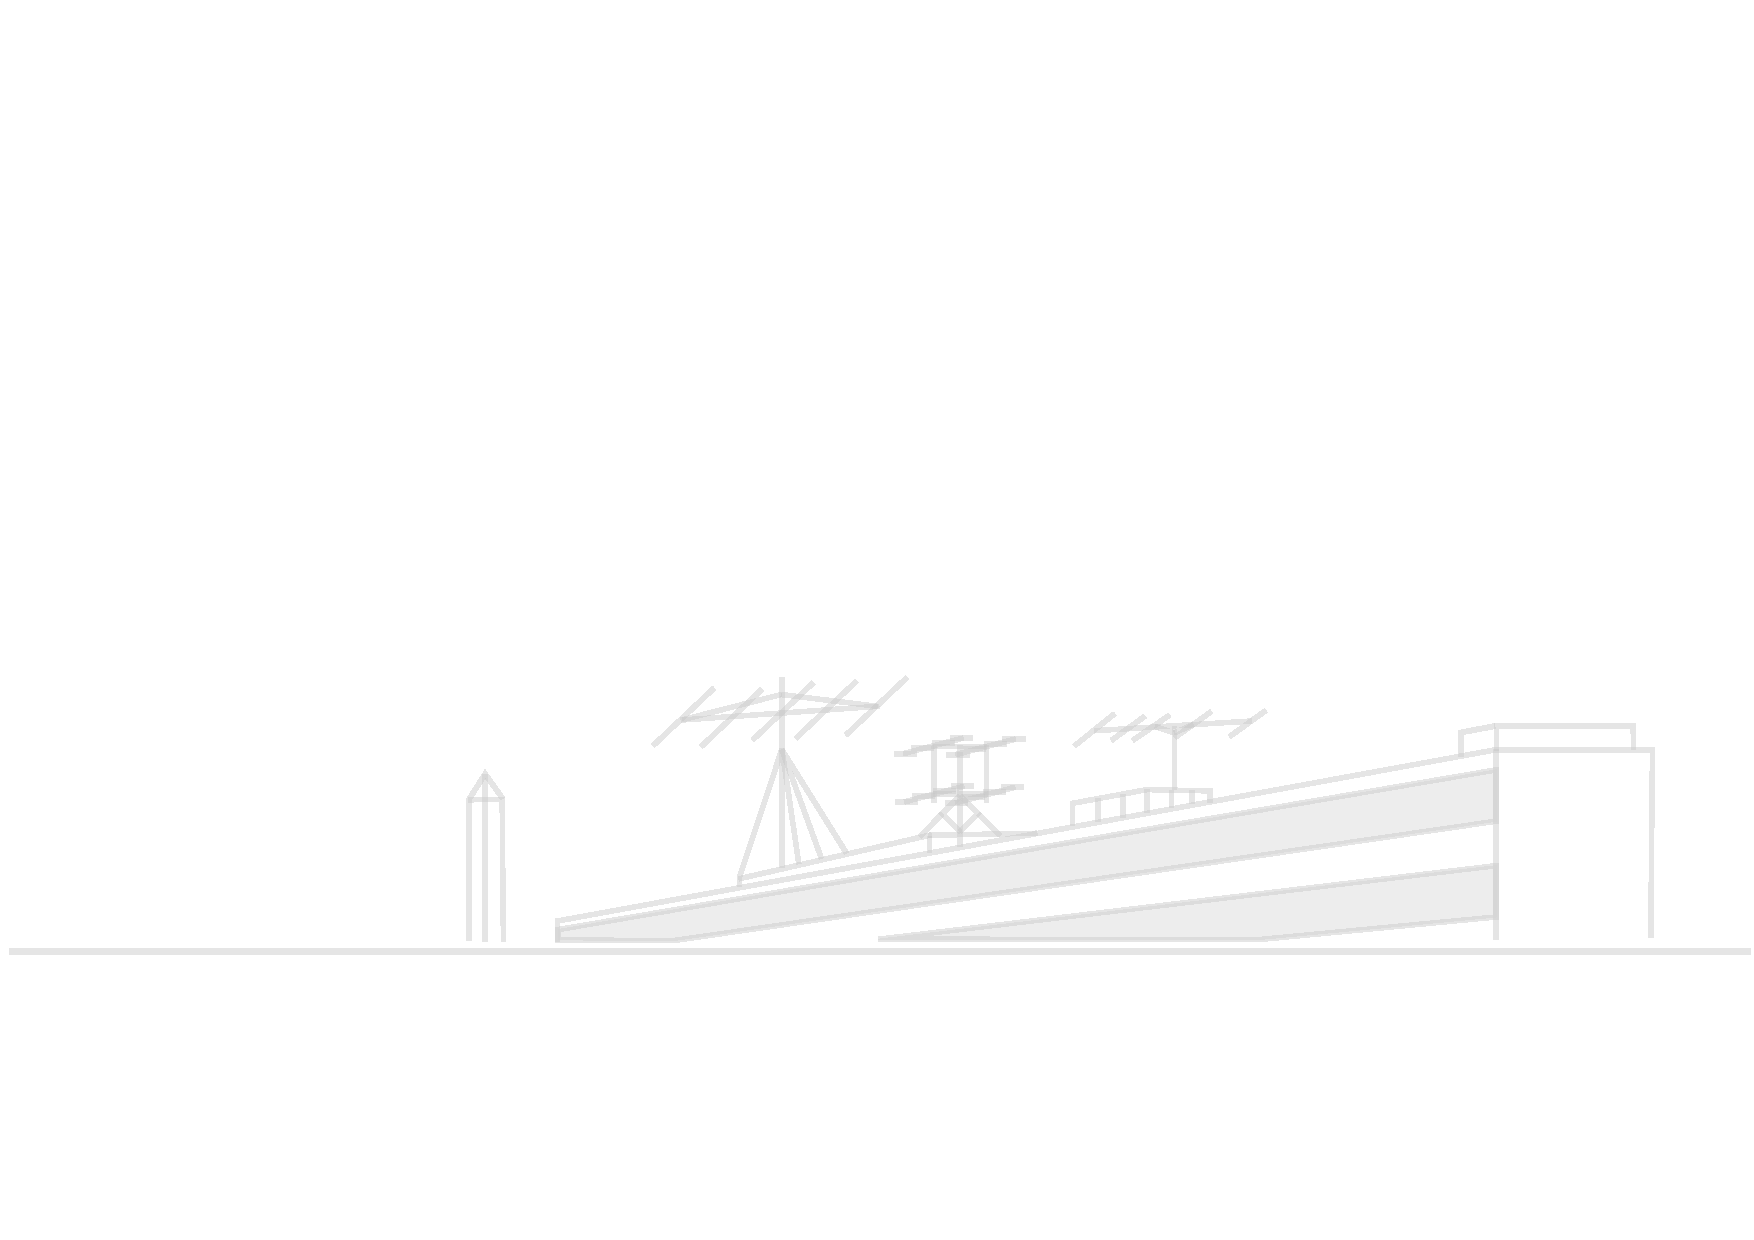
\includegraphics[width=17.8cm]{texdata/dk0tu_rooftop_background.pdf}
}

% Foliennummer einfügen
\setbeamertemplate{footline}[frame number]
%\setbeamertemplate{footline}{}

% Ändere das Zeichen vor jedem item
%\setbeamertemplate{itemize item}{\color{craneorange}$\blacktriangleright$}
%\setbeamertemplate{itemize subitem}{\color{craneorange}$\triangleright$}
%\setbeamertemplate{itemize subsubitem}{\color{craneorange}$\blacktriangleright$}

% Ändert die Blöcke 
\setbeamertemplate{blocks}[rounded][shadow=true]
% default | rounded [shadow=true|false]

%
% Eigene Kommandos
%

% Hack to get natbib and beamer working together. "The beamer user guide suggests
% that only the manual bibliography entry approach is supported"
% on some system it works out of the box, sometimes you need the hack :-(
% so check it --dl7bst
\ifdefined\newblock
    \relax
\else
    \newcommand{\newblock}{}
\fi

% \includedia command to generate png out of a dia file
% NEEDS installed dia and pdflatex option --shell-escape
\newcommand{\includedia}[1]{
    \immediate\write18{/usr/bin/dia #1.dia -e #1_diatmp.png -t png}
}

% RICHIG GROSSER FONT!
\newfont{\bigfont}{cmr10 at 144pt}
\newfont{\smallfont}{cmr10 at 8pt}

% Römische Ziffern
\makeatletter
\newcommand{\rmnum}[1]{\romannumeral #1}
\newcommand{\Rmnum}[1]{\expandafter\@slowromancap\romannumeral #1@}
\makeatother

% Schwarze Überschrift
%\setbeamercolor{frametitle}{fg=black}
%\setbeamercolor{title}{fg=black}

% Item- und Box-Farben
\definecolor{deepBlue}{HTML}{000066}
\setbeamercolor{itemize item}{fg=deepBlue}
\setbeamercolor{itemize subitem}{fg=deepBlue}
\setbeamercolor{description item}{fg=deepBlue}
\setbeamercolor{block title}{fg=deepBlue!100, bg=blue!15}
\setbeamercolor{block body}{fg=black, bg=blue!5}
\setbeamercolor{block title alerted}{fg=deepBlue, bg=red!75}
\setbeamercolor{block body alerted}{fg=black, bg=red!15}
\setbeamercolor*{block title example}{fg=blue!50, bg=blue!10}
\setbeamercolor*{block body example}{fg= blue, bg=blue!5}

%\setbeamercolor{section in head/foot}{parent=palette primary}
%\setbeamercolor{subsection in head/foot}{parent=palette secondary}
%\setbeamercolor{sidebar}{fg=darkblue,bg=yellow!90!orange}
%\setbeamercolor{title in sidebar}{fg=darkblue}
%\setbeamercolor{author in sidebar}{fg=darkblue}
%\setbeamercolor{section in sidebar}{fg=darkblue!10!black}
%\setbeamercolor{subsection in sidebar}{fg=darkblue!50!black}

% Titlepage Infos
\title{AFu-Kurs nach DJ4UF}
\author[DKØTU]{DKØTU\\ \footnotesize{Amateurfunkgruppe der TU Berlin}}
\institute[DKØTU]{\url{http://www.dk0tu.de} }

% PDF-Eigenschaften
\subject{DK0TU-Amateurfunkkurs nach DJ4UF}
\keywords{Amateurfunk Kurs HAM Radio Course CC-BY-NC-SA OpenSource TU Berlin DK0TU}

\subtitle{Betriebstechnik/Vorschriften 08: \\
  Amateurfunkstellen \\[2em]}
\date{Stand 14.11.2016}
 \begin{document}

\begin{frame}
    \titlepage
    \vfill
    \begin{center}
        \ccbyncsaeu\\
        {\tiny This work is licensed under the \em{Creative Commons Attribution-NonCommercial-ShareAlike 3.0 License}.}\\[0.5ex]
         \tiny Amateurfunkgruppe der Technische Universität Berlin (AfuTUB), DKØTU
         %\includegraphics[scale=0.5]{img/DK0TU_Logo.pdf}
    \end{center}
\end{frame}


\section[]{Einleitung}

\begin{frame}
  \frametitle{Einleitung: Amateurfunkstellen}

  \begin{center}
    \Large{Was ist eine Amateurfunkstelle?}
  \end{center}

\end{frame}

\section{Definition}

\begin{frame}
  \frametitle{Definition Amateurfunkstelle}

  Laut \textbf{Radio Regulations} (VO Funk), des \textbf{AFuG} und \textbf{Captain
  Obvious}: \\[2em]

  \begin{center}
    ``Eine Amateurfunkstelle ist eine Funkstelle des Amateurfunkdienstes.''
  \end{center}

\end{frame}

\begin{frame}
  \frametitle{Definition Funkstelle}

  Funkstelle im Sinne des Gesetzes:
  \begin{quote}
    Ein oder mehrere Sender oder Empfänger oder eine Zusammenschaltung von
    Sendern und Empfängern einschließlich der Zusatzeinrichtungen, die zum
    Ausüben eines Funkdienstes
    an einem Ort erforderlich sind.
  \end{quote}
  \\[3em]

  \uncover<2>{
  \begin{center}
    \Large Ahja! ;-)
  \end{center}
  }

\end{frame}

\begin{frame}
  \frametitle{Unterscheidungsmerkmale der Rufzeichen}

  Wie bereits in \texttt{BV06 (Rufzeichen - Landeskenner)} angedeutet, lassen
  sich die Rufzeichen, meist Präfixe, feiner untergliedern.\\[2em]

  In Deutschland gilt der Rufzeichenplan laut Verfügung Nr. 12/2005 geändert
  durch Verfügung Nr. 34/2005 der
  Bundesnetzagentur\footnote{\ExternalLink\url{http://www.bundesnetzagentur.de/SharedDocs/Downloads/DE/Sachgebiete/Telekommunikation/Unternehmen_Institutionen/Frequenzen/Amateurfunk/AmtsblattverfuegungenAFu/Vfg122005ge228ndertdurcId1833pdf.pdf?__blob=publicationFile&v=4}}.

\end{frame}

\subsection{Ausbildungs\-stationen}

\begin{frame}
  \frametitle{Ausbildungsstationen}

  \textbf{DN1--DN6}: Ausbildungsrufzeichen Klasse A \\
  \textbf{DN7--DN8}: Ausbildungsrufzeichen Klasse E

  \begin{itemize}[<+->]
    \item in DL \textbf{personengebunden}, nicht für Klubstationen
    \item \emph{aber} grundsätzlich nur vom \textbf{Auszubildenden} mit
      \textbf{Logbuch}führung zu verwenden und vom Ausbilder zu bestätigen
    \item nur in Anwesenheit und unter \textbf{Anleitung} des Ausbilders benutzen
    \item Ausbildungsfunkbetrieb im \textbf{Berechtigungsumfang} der
      Rufzeichenzuteilung (Klasse A oder E)
    \item kostenpflichtige unbefristete Erteilung durch die BNetzA
    \item \emph{nicht} für das alleinige Vorführen von Amateurfunkverkehr,
      sondern für OP mit Prüfungsabsicht
  \end{itemize}

\end{frame}

\subsection{Clubstationen}

\begin{frame}
  \frametitle{Clubstationen I}

  Klasse A: \textbf{DAØ, DA3, DFØ, DKØ, DLØ, DP3--9, DQ, DR} \\
  Klasse A mit nur einstelligem Suffix: \textbf{DA3, DP3--9, DQ, DR} \\
  Klasse A an exterritorialen Standorten: \textbf{DPØ--1} \\[1.5em]
  Klasse E: \textbf{DNØ}\footnote{18 Rufzeichen vergeben, Stand 10/2016} \\
  Klasse E mit nur einstelligem Suffix: \textbf{DA7--9}\\
  Klasse E an exterritorialen Standorten: \textbf{DP2} \\[2em]

  Für gemeinsame Aktivitäten von Gruppen. Z.B. DKØTU, Amateurfunkgruppe der
  \emph{TU Berlin} oder DAØCCC als Clubstation des \emph{CCC}. :-)

\end{frame}

\begin{frame}
  \frametitle{Clubstationen II}

  \begin{itemize}[<+->]
    \item ebenfalls \textbf{personengebunden} mit einem Verantwortlichen
      \footnote{Operator mit Call - gesetzl.: Person mit Zulassung zur
      Teilnahme am Amateurfunkdienst nach § 3 Abs. 1 AFuG}
    \item BNetzA stellt Club Calls kostenpflichtig aus
    \item jeder \textbf{Operator} muss Inhaber einer Zulassung zur Teilnahme am
      Amateurfunkdienst sein
    \item \textbf{Betriebsrechte} abhängig von Zulassung zur Teilnahme am
      Amateurfunkdienst\footnote{nach § 3 Abs. 1 AFuG}, auch bei Ausbildungsfunk
    \item kurzzeitige Standortänderungen müssen der BNetzA nicht angezeigt
      werden, z.B. Fieldday
    \item Clubstationen fallen \textbf{nicht} in CEPT-Empfehlung \textbf{T/R
      61-01} - Beantragung einer \textbf{Gastgenehmigung} notwendig!
  \end{itemize}

\end{frame}

\subsection{Kurzzeit-Sonderstationen}

\begin{frame}
  \frametitle{Kurzzeit-Sonderstationen}

  \textbf{DAØ} -- Kurzzeit-Sonderrufzeichen
  \footnote{Nicht zu verwechseln mit Sonder-DOK's}\\[1em]

  Für besondere Anlässe: Messen, Ausstellungen, Jubiläen, ... \\[3em]

  Wie beantragen? ... Richtig, einfach so mit einem Formblatt und
  kostenpflichtig bei der BNetzA.

\end{frame}

\section{Automatisch arbeitenden Amateurfunkstellen}

\begin{frame}
  \frametitle{Automatisch arbeitenden Amateurfunkstellen}

  \textbf{DBØ} - Relaisfunkstellen (\& Digipeater), Funkbaken \\[1em]

  offizieller Sprachgebrauch: ``\textbf{fernbediente oder automatisch arbeitende
  Amateurfunkstelle}'' \\[3em]

  Einschub an der Tafel: Funktionsprinzipien in Kürze, genauer dann in
  \texttt{BV10} und \texttt{BV11}

\end{frame}

\subsection{Relaisfunkstellen}

\begin{frame}
  \frametitle{Relaisfunkstellen (\& Digipeater) I}

  Laut \texttt{AFuV}: \\[1em]

  \begin{quote}
    Eine ``Relaisfunkstelle'' ist eine fernbediente Amateurfunkstelle
    (auch in Satelliten), die empfangene Amateurfunkaussendungen, Teile davon
    oder sonstige eingespeiste oder eingespeicherte Signale fern ausgelöst
    aussendet und dabei zur Erhöhung der Erreichbarkeit von Amateurfunkstellen
    dient.
  \end{quote}
  *gähn*

\end{frame}

\begin{frame}
  \frametitle{Relaisfunkstellen (\& Digipeater) II}

  \begin{itemize}[<+->]
    \item Notwendig: \textbf{Rufzeichenzuteilung} - BNetzA macht das gern...
      und besonders kostenpflichtig
    \item max. zulässige Strahlungsleistung $>30 MHz$: \textbf{15 Watt
      ERP}\footnote{Effective radiated power, die effektive
      Sendeleistung eines Senders plus Antennengewinn -- mehr in
      \texttt{E18}}
    \item Inhaber jederzeitige \textbf{Abschaltung} sicherstellen
    \item Betrieb nur auf ausgewiesenener \textbf{QRG} der Rufzeichenzuteilung
    \item Für Frage VD511: Lang andauernder Funkverkehr über ein Relais
      ist \emph{keine} Störung\footnote{im Sinne des § 13 Abs. 4 AFuV}
    \item Für Frage VA204: Relais \emph{nicht} zwischen 27120 und 27410 kHz
      \footnote{CB-Funk - Amateurfunk zwischen 28 MHz und 29,7 MHz}
  \end{itemize}

\end{frame}

\subsection{Funkbaken}

\begin{frame}
  \frametitle{Funkbaken}

  Baken dienen der Beobachtung der \textbf{Ausbreitungsbedingungen} -- sie
  wiederholen in regelmäßigen Abständen ihre Kennung auf fester \textbf{QRG}
  an festem \textbf{Standort}. \\[2em]

  Laut \texttt{AFuV}:
  \begin{quote}
    Eine ``Funkbake'' ist eine automatisch arbeitende Amateurfunk-Sendeanlage
    (auch in Satelliten), die selbsttätig Aussendungen zur
    Feldstärkebeobachtung oder zu Empfangsversuchen erzeugt.
  \end{quote}

\end{frame}

\begin{frame}
  \frametitle{Funkbaken: Grundlegende Gemeinsamkeiten I}

  Inhalt:

  \begin{itemize}
    \item Call
    \item Locator bei VHF/UHF
    \item ggf. weitere Informationen
  \end{itemize}

\end{frame}

\begin{frame}
  \frametitle{Funkbaken: Grundlegende Gemeinsamkeiten II}

  Vorraussetzungen:

  \begin{itemize}
    \item Amateurfunkzulassung
    \item standortbezogene Verträglichkeitsuntersuchung für QRGs
    \item wie gehabt: Bake muss kostenpflichtig beantragt werden
  \end{itemize}

\end{frame}

\begin{frame}
  \frametitle{Funkbaken: Grundlegende Gemeinsamkeiten III}

  \begin{center}
    Für alle: \\[2em]
    \Large Auf den QRGs kein Sendebetrieb!
    \footnote{Mehr dann in \texttt{BV09} (Betriebsarten, Sendearten, Frequenzen)}
  \end{center}

\end{frame}

\begin{frame}
  \frametitle{Funkbaken: VHF/UHF}

  Baken im VHF/UHF-Bereich (Region 1):

  \begin{itemize}
    \item VHF: 144,400 - 144,490 MHz
    \item UHF: 432,800 - 432,990 MHz
  \end{itemize}

\end{frame}

\begin{frame}
  \frametitle{Funkbaken: IARU Bakensystem}

  Globales HF Bakensystem \textbf{IBP}\footnote{International Beacon Project}
  mit 18 Baken nach festem Sendeplan:

  \begin{itemize}
    \item Zyklus: 3min
    \item QRGs 14100, 18110, 21150, 24930 und 28200 kHz
      \footnote{Deshalb nach IARU-Empfehlung vorgesehen und freizuhalten: \\
      \scriptsize 14099-14101, 18109-18111, 21149-21151, 24929-24931, 28190-28225 kHz}
    \item Call + 4x Träger: 100, 10, 1 und 0,1 Watt
  \end{itemize}

  \begin{center}
    Hörbeispiel: \Large \texttt{4U1UN} \hyperlink{refs}{\cite{ibp}}
  \end{center}

\end{frame}

\begin{frame}
  \frametitle{Funkbaken: IARU Bakensystem\hyperlink{refs}{\cite{ibp}} (tabellarisch)}

  \begin{center}
    \scriptsize
    \begin{tabular}{|l|l|l|l|l|l|l|}\hline
      Call   & Location                          & 14100 & 18110 & 21150 & 24930 & 28200 \\ \hline \hline
      4U1UN  & United Nations                    & 00:00 & 00:10 & 00:20 & 00:30 & 00:40 \\ \hline
      VE8AT  & \only<1>?\only<2>{Canada}         & 00:10 & 00:20 & 00:30 & 00:40 & 00:50 \\ \hline
      W6WX   & \only<1>?\only<2>{United States}  & 00:20 & 00:30 & 00:40 & 00:50 & 01:00 \\ \hline
      KH6WO  & \only<1>?\only<2>{Hawaii}         & 00:30 & 00:40 & 00:50 & 01:00 & 01:10 \\ \hline
      ZL6B   & \only<1>?\only<2>{New Zealand}    & 00:40 & 00:50 & 01:00 & 01:10 & 01:20 \\ \hline
      VK6RBP & \only<1>?\only<2>{Australia}      & 00:50 & 01:00 & 01:10 & 01:20 & 01:30 \\ \hline
      JA2IGY & \only<1>?\only<2>{Japan}          & 01:00 & 01:10 & 01:20 & 01:30 & 01:40 \\ \hline
      RR9O   & \only<1>?\only<2>{Russia}         & 01:10 & 01:20 & 01:30 & 01:40 & 01:50 \\ \hline
      VR2B   & \only<1>?\only<2>{Hong Kong}      & 01:20 & 01:30 & 01:40 & 01:50 & 02:00 \\ \hline
      4S7B   & Sri Lanka                         & 01:30 & 01:40 & 01:50 & 02:00 & 02:10 \\ \hline
      ZS6DN  & South Africa                      & 01:40 & 01:50 & 02:00 & 02:10 & 02:20 \\ \hline
      5Z4B   & Kenya                             & 01:50 & 02:00 & 02:10 & 02:20 & 02:30 \\ \hline
      4X6TU  & Israel                            & 02:00 & 02:10 & 02:20 & 02:30 & 02:40 \\ \hline
      OH2B   & \only<1>?\only<2>{Finland}        & 02:10 & 02:20 & 02:30 & 02:40 & 02:50 \\ \hline
      CS3B   & Madeira                           & 02:20 & 02:30 & 02:40 & 02:50 & 00:00 \\ \hline
      LU4AA  & \only<1>?\only<2>{Argentina}      & 02:30 & 02:40 & 02:50 & 00:00 & 00:10 \\ \hline
      OA4B   & \only<1>?\only<2>{Peru}           & 02:40 & 02:50 & 00:00 & 00:10 & 00:20 \\ \hline
      YV5B   & \only<1>?\only<2>{Venezuela}      & 02:50 & 00:00 & 00:10 & 00:20 & 00:30 \\ \hline
    \end{tabular}
  \end{center}

\end{frame}

\begin{frame}
  \frametitle{Funkbaken: IBP Live Karte und mehr}

  \begin{itemize}
    \item Live-Aktivitätskarte der IARU-Baken\footnote{\ExternalLink\url{http://www.dl1dlf.de/beacons.php}}
    \item Weltweite Liste von ca. 700 HF Beacons\footnote{\ExternalLink\url{http://dl8wx.de/baken_kw.htm}}
  \end{itemize}

\end{frame}

\section{Besondere Amateurfunkstellen}

\subsection{Besondere Studien}

\begin{frame}
  \frametitle{Besondere Studien}

  \textbf{DA4--5} - Amateurfunkstelle für besondere experimentelle und
  technisch-wissenschaftliche Studien nach \texttt{§16 Abs. 2 der AFuV}.

\end{frame}

\subsection{Exterritorial}

\begin{frame}
  \frametitle{Exterritorial}

  \textbf{DP0--2} - exterritorialen Gebiete, z.B.:

  \begin{itemize}
    \item Polargebiete
    \item Satelliten
    \item Botschaften
  \end{itemize}

  \begin{exampleblock}{Zugewiesene exterritoriale Clubstationen}
    \begin{description}
      \item[DPØISS] Weltraumstation ISS
      \item[DPØGVN] Neumayer-Station Antarktis
      \item[DP1POL] Weitere Antarktis Station
    \end{description}
  \end{exampleblock}

\end{frame}

\subsection{Fuchsjagd}

\begin{frame}
  \frametitle{Fuchsjagd}

  \textbf{Peilkennungen} in Morsecodierung für Fuchsjagdsender\footnote{weniger als 5 Watt
  Senderleistung - meist $80m$ und $70cm$} (keine Rufzeichen\footnote{M = Großbritannien}!):

  \begin{itemize}
    \item \textbf{MO}
    \item \textbf{MOE}
    \item \textbf{MOI}
    \item \textbf{MOS}
    \item \textbf{MOH}
    \item \textbf{MO5}
  \end{itemize}

\end{frame}

\section[]{Präfix-Quiz}

\begin{frame}
  \frametitle{Präfix-Quiz}

  \begin{exampleblock}{
    \LARGE
    \begin{center}
      \only<1-2>{DP1, DPØ \\}
      \only<3-4>{DBØ \\}
      \only<5-6>{DO1-9 \\}
      \only<7-8>{DFØ, DKØ, DLØ \\}
      \only<9-10>{DN1-9 \\}
      \only<11-12>{DNØ \\}
      \only<13-14>{DAØ, DQ, DR \\}
      \only<15-16>{DA-DM \\}
      \only<17-18>{DA5U \\}
      \only<19-20>{MO, MOE, MOI, MOS \\}
    \end{center}
    }
    \Large
    \begin{center}
      \only<1,3,5,7,9,11,13,15,17,19>{...? \\}
      \only<2>{Exterritoriale Funkstelle \\}
      \only<4>{Relaisfunkstelle, Digipeater, Funkbake \\}
      \only<6>{Personengebunden Klasse E \\}
      \only<8>{Klubstation Klasse A \\}
      \only<10>{Ausbildungsstation \\}
      \only<12>{Klubstation Klasse E \\}
      \only<14>{Kurzzeitclubstation \\}
      \only<16>{Personengebunden Klasse A \\}
      \only<18>{Experimentelle Sonderstation \\}
      \only<20>{Peilkennungen für Fuchsjagdsender \\}
    \end{center}
  \end{exampleblock}

\end{frame}

\section[]{Zusammen\-fassung}

\begin{frame}
  \frametitle{Zusammenfassung}

  Komplette und korrekte Liste in den aktuellen Amtsblattverfügungen AFu der
  BNetzA\footnote{\ExternalLink\url{http://www.bundesnetzagentur.de/SharedDocs/Downloads/DE/Sachgebiete/Telekommunikation/Unternehmen_Institutionen/Frequenzen/Amateurfunk/AmtsblattverfuegungenAFu/Vfg122005ge228ndertdurcId1833pdf.pdf?__blob=publicationFile&v=4}}\\[2em]

  \dots oder etwas übersichtlicher in der Wikipedia\footnote{\ExternalLink\url{https://de.wikipedia.org/wiki/Amateurfunkrufzeichen}}

  %    Komplette Liste (nicht 100\%ig korrekt) nach DJ4UF\hyperlink{refs}{\cite{dj4uf}}:
  %    %todo korrigieren
  %
  %    \begin{itemize}
  %        \item Personengebunden Klasse A: DA bis DM
  %        \item Personengebunden Klasse E: DO1…DO9
  %        \item Klubstation Klasse A: (DB0), DF0, (DG0), DH0, DK0, DL0, DM0
  %        \item Klubstation Klasse E: DO0
  %        \item Ausbildungsstation: DN1-9
  %        \item Kurzzeit(klub)station: DA0, DQ, DR
  %        \item Exterritoriale Funkstelle: DP1, DP0
  %        \item Experimentelle Sonderstation: DA5U
  %        \item Relaisfunkstelle, Digipeater, Funkbake: DB0
  %    \end{itemize}

\end{frame}

\renewcommand{\refname}{Referenzen}

\begin{frame}
  \frametitle{Referenzen/Links}
  \hypertarget{refs}{}
  \footnotesize

  \begin{thebibliography}{}
    \bibitem{dj4uf} Moltrecht B/V 08: \\
      \url{https://www.darc.de/der-club/referate/ajw/lehrgang-bv/bv08/}
    \bibitem{wp}    Wikipedia DE: \\
      \url{http://de.wikipedia.org/wiki/Amateurfunkrufzeichen} \\
      \url{http://de.wikipedia.org/wiki/Ausbreitungsbake}
    \bibitem{ibp}   NCDXF/IARU Beacon Transmission Schedule: \\
      \url{http://www.ncdxf.org/beacon/beaconschedule.html}
    \bibitem{bpol}  Baken-Politik der IARU Region 1: \\
      \url{http://www.darc.de/referate/hf/baken/}
  \end{thebibliography}

\end{frame}

% Hier könnte noch eine Kontaktfolie stehen

\end{document}

